\chapter{Clustering}
\label{ch:clustering}

\section{K-means algorithm}
\label{sec:kmeans}

Let's assume to have extrapolated $F$ features from each of our signals, to produce a collection of $n$ snapshots $\snapshot_i, i \in [1,n]$ (every snapshot is a vector of features $\in \mathbb{R}^F$). The task is to define a set $\cluster$ of $k$ clusters ($k \leq n$) $\cluster_i, i \in [1,k], \cluster_i \in \cluster$ that minimize the squared sum of the distances between the snapshots and the centroids $\vect{c}_i$ of the clusters they belong to. This is equivalent to find the centroids that minimize the variance of the clusters themeself, so the problem can be formulated as in the \autoref{eq:kmeans_problem}.

\begin{equation}
  \argmin{\cluster}\sum_{i=1}^{k}\sum_{\snapshot_j \in \cluster_i} \norm{\snapshot_j - \vect{c}_i}^2 = \argmin{\cluster}\sum_{i=1}^{k}\abs{\cluster_i}\mathrm{Var}\cluster_i
\label{eq:kmeans_problem}
\end{equation}

Unfortunately, this problem is NP-hard, even for as little as $F=2$ features considered \cite{MAHAJAN201213}, so it is not possible to guarantee to find the global optimum in a reasonable time. 

Anyway, clustering algorithms were already developed in the 1950s, and the most famous one was the K-means algorithm. The first appearence of the therm \quoted{K-means} was used in 1957 by MacQueen \cite{macqueen1967some}, and the algorithm settled to a \quoted{standard} version in 1982 \cite{Lloyd1982}.

Nowadays, the K-means algorithm is one of the most used clustering algorithms, and it is implemented in many libraries, such as \texttt{scikit-learn} for \texttt{Python}, and others for \texttt{C}, \texttt{R}, \texttt{MATLAB}, etc. However, the runtime performances vary widely depending on the implementation \cite{Kmeans-performances-Kriegel2017}.


\subsection{Evaluation of a new instance}

At this point, with a model trained on the data, a generic $n$th new snapshot instance $\snapshot_n$ can be evaluated using the K-means algorithm.
From a geometric point of view, the snapshot $\snapshot_n$ is a point in the ${F}$-dimensional space, where ${F}$ is the number of features used to train the model.

For demonstration purposes, in this section, it is considered an example with ${F}=3$ features.

\begin{figure}[htbp]
  \centering
  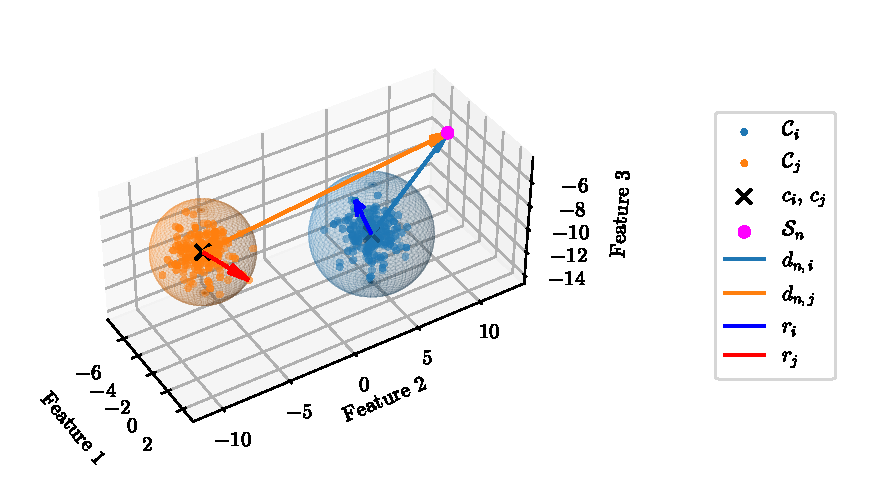
\includegraphics[width=\textwidth]{images/Spheres_2.pdf}
\caption{Cluster model in the $3$-dimensional space, with new snapshot $\snapshot_n$}
\label{fig:clust_spheres}
\end{figure}

In the \autoref{fig:clust_spheres}, the training data are represented in the $3$-dimensional space, where the axis are the features used to train the model. The K-means model has been ideally trained with an arbitrary number $k$ of clusters but, for display purposes, only two clusters  ($\cluster_i$ and $\cluster_j$) are plotted. 
\paragraph*{}
The entities shown in the \autoref{fig:clust_spheres} are:
\begin{itemize}
  \item $\vect{c}_{i(j)}$ is the centroid of the $i$th ($j$th) cluster;
  \item $\vect{r}_{i(j)}$ is the radius of the $i$th ($j$th) cluster, it is defined as the distance between the centroid $\vect{c}_{i(j)}$ and the farthest point belonging to the cluster itself;
  \item $\cluster_{i(j)}$ is the set of training snapshots belonging to the $i$th ($j$th) cluster, it has a centroid $\vect{c}_{i(j)}$ and a radius $\vect{r}_{i(j)}$;
  \item $\snapshot_n$ is the new snapshot to be evaluated;
  \item $\vect{d}_{n,i}$ is the vector between $\snapshot_n$ and $\vect{c}_i$;
  \item $\vect{d}_{n,j}$ is the vector between $\snapshot_n$ and $\vect{c}_j$;
  \item the semi-transparent spheres represent the cluster sizes, the radius of the spheres is the radius of the cluster itself, and the center is the centroid of the cluster;
\end{itemize}

\subsection{Assignation of the new instance to a cluster} 
The procedure for assigning the new snapshot $\snapshot_n$ to a cluster is quite simple, it is sufficient to compute the distance between $\snapshot_n$ and the centroids $\vect{c}_m$, $\forall m \in  [1, \dots , k]$. The distance is defined as the $l^2$-norm in the feature space, and can be computed using the \autoref{eq:clust_dist}, and assign $\snapshot_n$ to the cluster with the minimum distance.

\begin{equation}
  \label{eq:clust_dist}
  \vect{d}_{n,m} = ||\snapshot_{n,f} - \vect{c}_{m,f}||_2 = \sqrt{\sum_{f=1}^{F} (\snapshot_{n,f} - \vect{c}_{m,f})^2}
\end{equation}

\subsection{Evaluation of the new instance}
Once the new snapshot $\snapshot_n$ has been assigned to the right cluster $\cluster_i$, some kind of measure (a.k.a. metric) linked to how novel this snapshot is needs to be computed. In this document, this measure, referred to the $n$-th cluster, will be called $e_n$, in order to remind some sort of error, even if it is not an error in the strict sense. One simple approach could be to compute the difference between the distance of $\snapshot_n$ from the centroid $\vect{c}_i$ and the radius $\vect{r}_i$ of the cluster itself. With this approach, the measure defined in the \autoref{eq:clust_eval} is relative to the current snapshot, so it is possible to use that as a novelty measure.

Few consideration about the resoult of the \autoref{eq:clust_eval}:
\begin{itemize}
  \item if $e_{n} > 0$, the new snapshot $\snapshot_n$ is outside the sphere of radius $\vect{r}_i$ centered in $\vect{c}_i$, so it is probably a novel snapshot;
  \item if $e_{n} < 0$, the new snapshot $\snapshot_n$ is inside the sphere of radius $\vect{r}_i$, so it is probably a normal snapshot. In this case it is worth noticing that this assumption is reasonable only if the shape of the point cloud resambles a sphere, otherwise the radius $\vect{r}_i$ is not a good measure of the cluster size, and use it for novelty detection would not be reasonable. \emph{This enpasises the importance of the standardization procedure applied to the features before the training phase};
\end{itemize}

\begin{equation}
  \label{eq:clust_eval}
  e_{n} = ||\vect{d}_{n,i}||_2 - ||\vect{r}_{i}||_2, \text{ where $i$ is the of the assigned cluster}
\end{equation}

Using this metric it is possible to define as novelty all the snapshots with $e_{n} > 0$, and as normal all the snapshots with $e_{n} < 0$. This approach is not very robust because s snapshot that is even slightly outside the sphere of radius $\vect{r}_i$ will be considered as novelty, but since the sphere is tuned the training \emph{measured} data, that have an aleatory component, this approach will probably detect some novelty even in normal snapshots.

\subsection{Evaluation of the new instance with a threshold}
In order to improve the robustness of the novelty detection algorithm, it is possible to define a threshold ${t}_i$ for each cluster $\cluster_i$, and use it to detect the if a snapshot is a novelty or not. Once the threshold ${t}_i$ is defined, the detection of the novelty can be triggered by the condition $e_{n} > \norm{\vect{r}_i}+ {t}_i$.

\paragraph*{}
At this point the problem is that the user would have to define a threshold for each cluster, and this is not a trivial task. This is because it is likely that the clusters have different sizes, and so one threshold for all the clusters would be more conservative for the smaller clusters and less conservative for the bigger ones.

To address this problem, it is possible to change the definition of the metric itself, so that is not dependent on the cluster size. This can be done by normalizing the already defined metric $e_{n}$ with the radius $\vect{r}_i$ of the cluster itself, as shown in the \autoref{eq:clust_eval_norm}. In this way, $t_i$ can be defined as a percentage of the cluster size, so that the user can define a single threshold for all the clusters, and selecting the number to assign to $t_i$ has a more intuitive meaning. From now on if not otherwise specified, the metric $e_{n}$ will be this normalized version. 
Obviously, the metric can be easily displayed as a percentage: $e_{n,\%} = e_n \cdot 100$.
This value can be evaluated in real-time, and plotted in a graph so that the user can see the novelty metric behavior over time.

\begin{equation}
  \label{eq:clust_eval_norm}
  e_{n} = \frac{\norm{\vect d_{n,i}}-\norm{\vect r_{n,i}}}{\norm{\vect r_{n,i}}} = \frac{\norm{\vect{d}_{n,i}}}{\norm{\vect{r}_{i}}} - 1, \text{ where $i$ is the of the assigned cluster}
\end{equation}

\subsection{Evaluation procedure}
All said in the previous sections can be summarized in the following procedure:

\begin{algorithm}
  \caption{Evaluation of a new snapshot with a K-means model}
  \label{alg:eval_new_snapshot}
  \begin{algorithmic}[1]
  \Procedure{eval}{$\mathcal{M}_{\text{\texttt{k-means}}},\snapshot, t$}
  \LineComment{$\mathcal{M}_{\text{\texttt{k-means}}}$ is the trained K-means model}
  \LineComment{the model contain the centroids $\vect{c}_i$ and the radii $\vect{r}_i$ of the clusters}
  \LineComment{$\snapshot$ is the new snapshot to be evaluated}
  \LineComment{$t$ is the threshold for the novelty detection}
  \State $k \gets \text{number of clusters in $\mathcal{M}_{\text{\texttt{k-means}}}$}$
  \State min $\gets \infty$ \Comment {initialize the minimum distance}
  \For{$i \gets 1$ to $k$}
    \State $\vect{d}_{i} \gets \snapshot - \vect{c}_{i}$
    \If {$\norm{\vect{d}_{i}} < \text{min}$}
      \State min $\gets \norm{\vect{d}_{i}}$
      \State $i_{\text{min}} \gets i$
    \EndIf
    \EndFor
  \State$e \gets \frac{\norm{\vect{d}_{i_{\text{min}}}}}{\norm{\vect{r}_{i_{\text{min}}}}} - 1$ \Comment {compute the novelty metric}
  \If {$e > t$}
    \State \Return novelty  \Comment {the snapshot is novelty}
  \Else
    \State \Return normal \Comment {the snapshot is normal}
  \EndIf
  \EndProcedure
  %\end{small}
  \end{algorithmic}
  \end{algorithm}